\chapter{考察}
本章ではReaderLintを試験的に運用して得られたフィードバックや問題点をもとに考察を行う

\newpage

\section{評価}

本章では実装したReaderLintを実際に運用し,利用したユーザーからのフィードバックを評価として述べる.

\subsection{筆者の運用,利用における意見}
筆者を含め,ReaderLintを体験してもらった.主にReaderLintを用いた場面は
Twitter(TweetDeck)\footnotemark[1]\label{twitter},
Note \footnotemark[2]\label{note},
はてなブログ \footnotemark[3]\label{hatenablog} 
といったテキストを読む行為が主体であるWebサービスである.
以下は今回体験したユーザーからの文章レイアウトを変更することに関してのフィードバックの一例である.

\footnotetext[1]{
    引用元 \protect\url{
        https://tweetdeck.twitter.com/
    }
}
\footnotetext[2]{
    引用元 \protect\url{
        https://note.com/
    }
}
\footnotetext[3]{
    引用元 \protect\url{
        https://hatenablog.com/
    }
}
\subsubsection{文章を見失わずに読める}
文章のつながりが分かりやすいため,文末と次行の文頭の前後関係の判断が行いやすく,
文章の文頭を見失うことが少なかったという意見を得た.
これは第2章にて紹介した小林らによる論文でも有意性を示していた視認性の向上を示した評価であると考えられる.

つづいて,DOMサイズが大きい,つまりは横幅の大きいゆえに一行の文字数が長くなるテキストに対して,
横幅が900pxを超えたDOMに対し横幅を900px以下に収まるよう処理を加えたところ,視認性が向上したように思えた,
という意見を得た.これは一行における文字が多いため,元の文章自体の視認性がもともと低かった場合に対して
視野内に収まりやすくしたことが要因である,と推測する.
これも第2章で述べられた行末と次行の行頭を追うためのサッケード
距離が短くなったために文章を追うことができるようになった,
という眼球運動のフォローとなった結果ではないか,と考える.

\subsubsection{両端揃えでない文章への違和感}
横書きの文章に対して左端のみならず右端も揃った,つまりは活字媒体の校正ルールである
横組版に沿った両端揃えではない文章レイアウトに違和感を覚える,という意見があった.
改行を意図的に行なうレイアウトと右詰されていない文章とを両立するのは難しく,
設定する場合にはCSSを用いたスタイル変更を用いることになる.(text-align-all:justify)
この方法による両端揃えは両端揃えの調整が必要になった際,字間を大きくすることにより行末まで詰める仕様になっている.
%画像あったほうがいいかも
\begin{figure}[H]
    \centering
    \label{fig:ryohashi}
    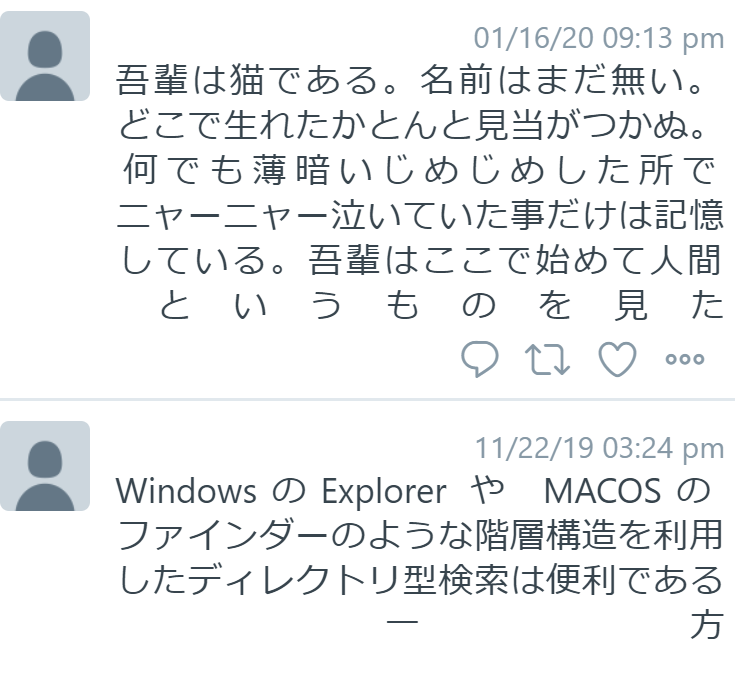
\includegraphics[width=0.5\columnwidth]{image/04/img1.png}
    \caption[両端揃えを行なった文章レイアウト] {両端揃えを行なった文章レイアウト}
\end{figure}

そのため一行に含まれる文字数が少ない場合には字間が大きくとってしまい,文字と文字の間が開いて視認性を損ねる
可能性が生じてしまう.また,このような文章の字間を調整することで両端揃えを行う処理はアクセシビリティの観点から,字間が不規則になることで失読症患者など
認知問題を抱えた読み手にとって,問題があるレイアウトになってしまう,という報告がW3Cのガイドラインとしても掲げられている.\cite{WCAG2.0} 
ReaderLint側でも両端揃えの文章レイアウトに慣れているユーザーにとって凹凸があるとして違和感を持つ行末までの距離や閾値,
凹凸を少なくした文章レイアウトとそうではないものとを比較した上,視認性がどこまで失われたと感じられるのか,を踏まえた上で今後の懸念事項
として調節する機能拡張を行なっていきたい.

\subsubsection{文節の切り方によって二つの意味が生じる文章}
文節で文章を区切る,という改行方法はレイアウト側によって文意を
規定してしまうことが起こりえる,という意見もあった.
日本語における形態素解析や分かち書き処理の精度の向上は自然言語処理研究の課題でもあり,精度の向上を試みる研究がなされている.
例えば「この先生き残るにはどうすればいいか」というような例文があった場合に
「この/先/生き/」という区切り方と「この/先生/」という区切り方とでは文意が大きく異なってしまう.
ReaderLintにて使用しているTinySegmenterでこの文章の分かち書きを行なったテストでは,
以下画像のように後者の区切り方となった.
\begin{figure}[H]
    \centering
    \label{fig:seid}
    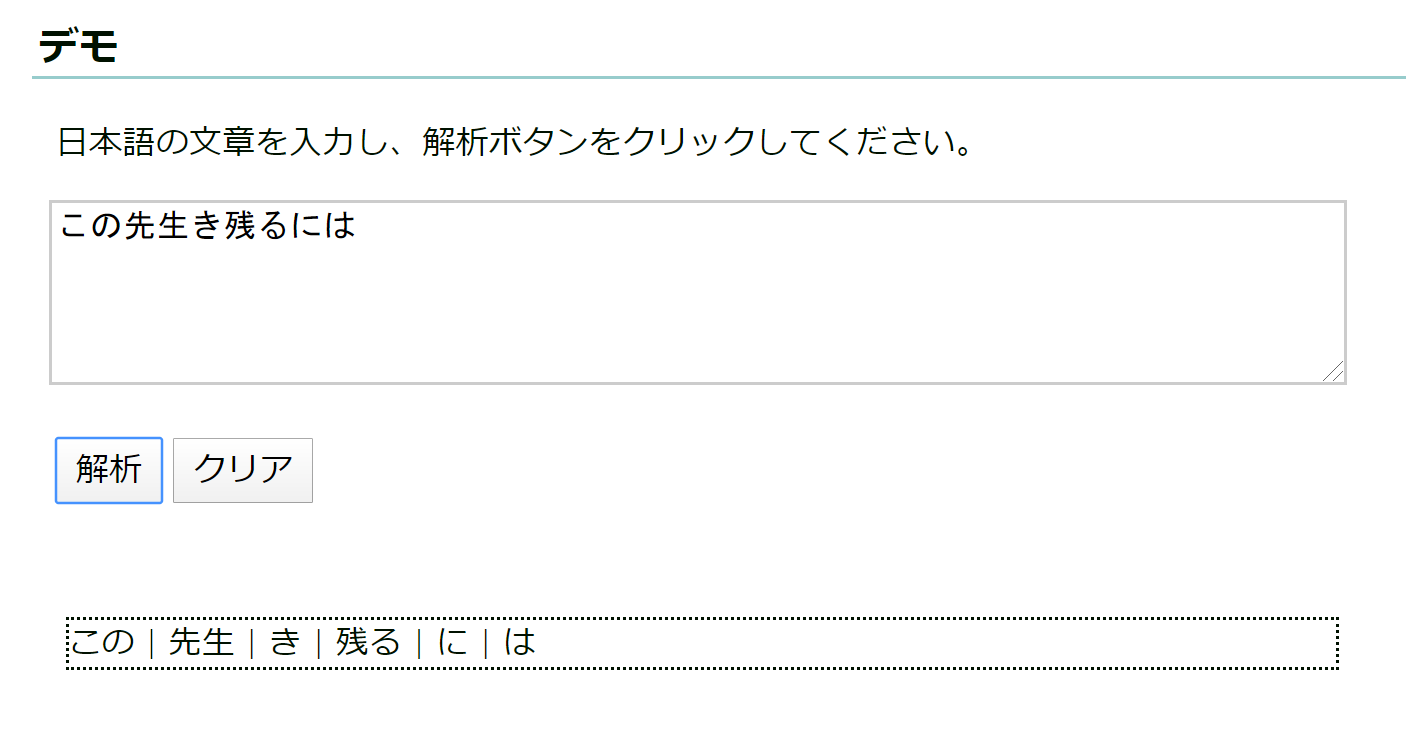
\includegraphics[width=0.7\columnwidth]{image/04/img2.png}
    \caption[TinySegmenterを用いた日本語分かち書きの精度] {TinySegmenterを用いた日本語分かち書きの精度}\footnotemark[1]
\end{figure}

\footnotetext[1]{使用サイト参照:
	\protect\url{http://chasen.org/~taku/software/TinySegmenter/}
}
このように書き手側の文意に問わず改行位置は日本語分かち書きに沿った文章として分かれるため,読み手が文意の誤読を起こしかねない.
この解決方法としてはより精度の高い分かち書きライブラリを用いることで精度を上げる方法がある.
辞書データ型の日本語分かち書きライブラリを用いることが挙げられる.今回はJavaScript製で辞書データを用いた
形態素解析ライブラリであるkuromoji.jsを用いて,先ほど入力したテキストを分かち書きすると以下のような結果となった.
\begin{figure}[H]
    \centering
    \label{fig:seid2}
    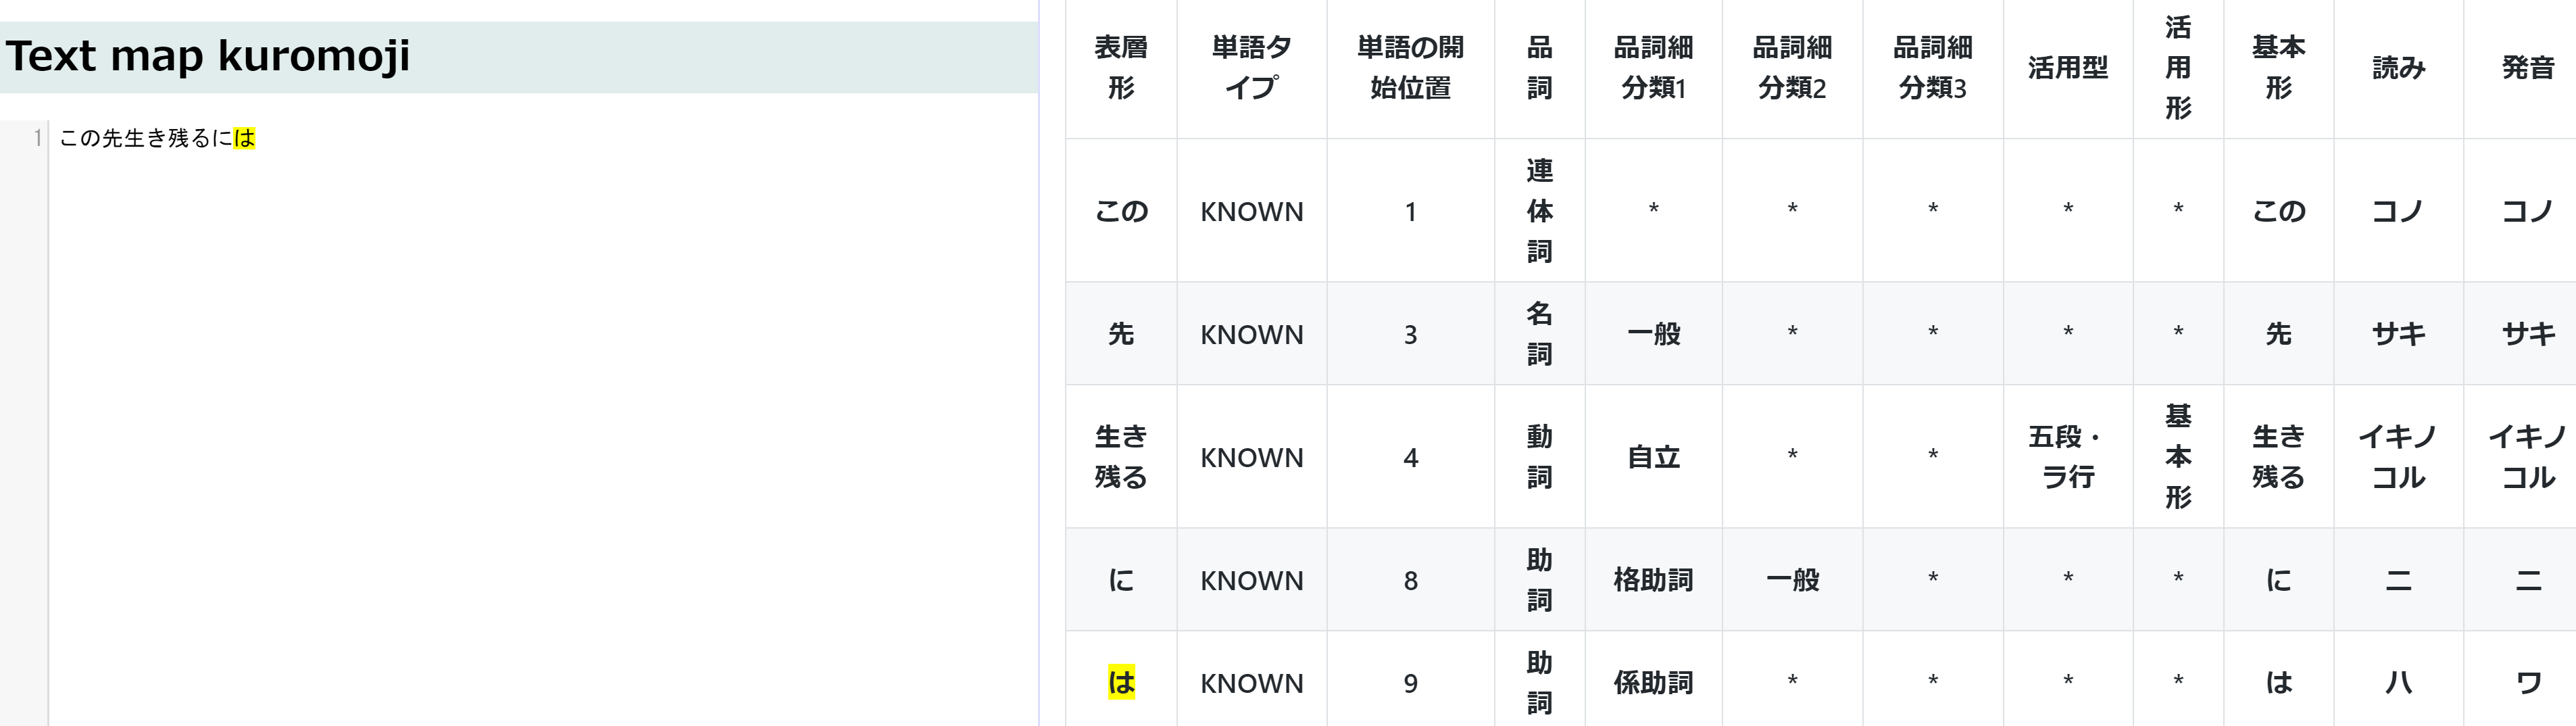
\includegraphics[width=0.7\columnwidth]{image/04/img3.png}
    \caption[kuromojiを用いた分かち書きの精度] {kuromojiを用いた分かち書きの精度}\footnotemark[2]
\end{figure}

\footnotetext[2]{使用サイト参照:
	\protect\url{https://azu.github.io/text-map-kuromoji/}
}

画像のように辞書データ依存の日本語分かち書きは文章として,文章に違和感のない分かち書きに成功している.
この一方で,第3章でも述べたように辞書データ型は辞書に載っていない,
たとえば,近年リリースされたコンテンツのタイトル名称等といった未知語を処理する際には不安定な結果を出力する場合がある.
このような未知語に対しての処理が対策が必要である.
一例をあげると,作品のタイトルを囲む際に用いられる二重括弧(例:『名探偵コナン』)で囲まれた文字列は1つの固有名詞として扱う,
などの日本語分かち書きする処理に対し,柔軟なルールを実装するといった配慮が必要があるだろう.また,ユーザー個人が多用するが辞書として登録されていない
単語等には新たに辞書データに単語を登録し学習することで未知語だった単語の検出率を上げる,といった方法も有効である.

\section{まとめ}
ReaderLintを運用したユーザーのフィードバック,およびそれを踏まえた考察を行なった上で改善策を述べた.
文節間改行レイアウトに関してはその視認性はすでに研究として着目され,その有用性を示されており,実際に視認性がよくなった,
というフィードバックが多かった一方,その対象となる文章が長いほど,従来の横組版とは異なる両端揃えでないことに
違和感を感じるフィードバックもあがっていた.また,自然言語処理系の特有の問題である分かち書きの精度の問題から,文章の意図を異なる解釈で
改行を行い,読み手に誤った認識を与えてしまう可能性も示唆された.